\documentclass[11pt]{article}
\usepackage[utf8]{inputenc}
\usepackage{geometry}
\geometry{a4paper, portrait, margin=2cm}
\usepackage[english]{babel} 
\usepackage{parskip}
\usepackage{chngcntr}
\counterwithin{figure}{section}
\usepackage{url}
\usepackage[noadjust]{cite}
\usepackage{mathtools}
\usepackage[nottoc,numbib]{tocbibind}
\usepackage{graphicx}
\usepackage{pdflscape, lscape}
\usepackage{array}
\usepackage{tabularx}
\usepackage{caption}
\usepackage{everypage}
\usepackage{enumitem}
\setlist{noitemsep}

\title{An Evaluation of Cooperative Handheld Robotics in a Simplified 3D Construction Environment}
\author{Chris Meehan}

\begin{document}

\begin{titlepage}
	\centering
	
	
\includegraphics[width=0.6\textwidth]{bristol.png}
	\vspace{2cm}

	{\huge\bfseries The Design and Evaluation of a Four Degree-Of-Freedom Cooperative Handheld Robotic Device in a Simplified 3D Construction Environment\par}
	\vspace{1.5cm}

	{\Large\itshape By Chris Meehan\par}
	
	Supervised by\par
	Dr. Walterio Mayol-Cuevas
	
	\vspace{1.5cm}
	
	Department of Computer Science\par
	University of Bristol

	\vfill

% Bottom of the page
	{\large \today\par}
\end{titlepage}


\tableofcontents

\pagebreak

\section{Abstract}

\section{Introduction}

\section{Handheld Robot Design}
\subsection{Flexible Robotic Arms}
\subsection{Design Process of Four Degrees-Of-Freedom Device}
\begin{itemize}
\item{The initial design took direction based on the use of four Hi-Tec MS7980 servomotors to provide a degree of freedom each, driving the arm via some form of lightweight cable.}
\item{A flexible foam tube was provided to act as the arm of the robot with outer diameter 42mm and inner diameter 19mm}
\item{Early design was based around a single solid part, where two servos were mounted at the back and another two slightly offset. A tubular section was also present to attach the foam arm. However, after attempting to 3D print this, the quality was severely hindered by the need for excessive scaffolding to support the overhanging elements of the design}
\item{As a result, the base was designed in two halves, with a separate piece for the tubular mount for the arm. These three parts could then be printed separately in an orientation that didn't result in any overhanging sections. As such, a much higher 3D print quality could be achieved.}
\item{At this point, alternate shapes were explored based around this fundamental design, with compactness being a priority. One such design would entail a cubic section, where all servomotors would be at the same level, reducing the required moment arm to hold the device}
\item{The cable management was then accounted for in order to drive the arm. Tubular linkages are attached to the arm with holes to connect the cables to the servomotors. When connecting the cables from the servomotors to the tubular linkages, the orientation of the cables in 3D space must be considered in order to determine how the arm will move in response to servomotor angle changes. Initially, the cables were planned to be connected in a straight line direct from the servomotor to the arm linkages, eliminating the need to account for friction}
\item{INSERT IMAGE OF THE CAD OF THE CUBIC DESIGN WITH CONNECTING LINES}
\item{However, by connecting the cables directly, in a manner with a relative angle between the axis of the arm, the motion of the arm in response to a servo angle change is unpredictable, and more importantly, a single servo motion may not necessarily constrain the arm to motion in a single degree of freedom. That is, the arm will move in one direction initially, resulting in a different angle between the cable and the arm, and further servo motion will cause movement along the axis of the cable (in a different direction to the initial motion). }
\item{As such, it was decided that a configuration was necessary that routed the cables so that each servo acts solely on a single degree of freedom, with the cables running parallel to the arm. This of course required changing the direction of the cables by passing them through guiding holes, accepting friction where they make contact with the edges of the holes.}
\item{Further iterations of the dimensions in the design were explored in order to find a configuration in which the cables of the rear pair of servos did not interfere at all with those of the front pair. Holes were implemented on the central tube holder pillar so that the cables could pass through in an orientation normal to the servo arms of the rear (so the driving force on the servo arm would be tangent to the radius  of the servo arm motion), meaning that motion from the servo would result in the maximum movement of the arm. If it was directed non-tangentially, motion from the servo would have less of an effect on the motion of the arm.} 
\item{PUT IN IMAGE OF SERVO ARM WITH CABLE ATTACHED TANGENTIALLY AND MOTION TO SHOW LARGE CORRESPONDING MOTION, AND THEN SIMILAR FOR ATTACHED AT AN ANGLE SHOWING LESS MOTION.}
\item{A similar approach was taken to guiding the cables of the front two servos by passing them through holes in the base mounting for the tube holder }
\item{Once the cables have been guided in such a way that they are perpendicular to the servo arms, they then required another set of holes in order to guide them along the axis of the arm. Therefore a faceplate with four guiding holes was fitted to the front of the housing.}
\item{A low friction fishing wire was thus selected as the cable material [INSERT REFERENCE TO PRODUCT??], and was found to move freely against the 3D printed PLA plastic with little signs of wear or grazing}
\item{An initial prototype was printed with relatively low percentage infill in order to test the concept. The medium sized servo arms that were supplied with the servo were used, feeding the cables through the set of holes along each side of the arm to lock it in place. Exiting the cable at the outermost hole gave an effective diameter (which acts on the cable) of 45mm, whereas the overall diameter of the servo arm was 52mm. Initially, this prototype was ran with all four servos connected to the respective arm linkages, achieving correct motion. This proved that the friction of the cables was not a cause for concern, and the routing of the cables was successful. However, the range of motion of the front two servos were limited by potential collision with the base mounting for the central tube holder, only affording 35 degrees either side of the neutral position. (the max range of the servos is 70 degrees either side but this should have been mentioned already.}
\item{Another issue found was the inconsistent rate of motion in a given degree of freedom with increasing servo angle, this is for similar reasons as explained earlier in FIGURE X [THE ONE SHOWING THE CABLE ATTACHED TANGENTIALLY TO THE SERVO ARM]. At larger angles, a similar movement of the servo arm results in a smaller response motion from the arm. Hence the effect is an overall reduced range of motion of the arm as high servo angles have minimal effect on the motion as they don't pull the cable further. The other key problem observed was that on the opposite side to the pulling action of the arm, the cable became slack. This is because as the arm flexes, the extra cable available afforded by the forward motion of this end of the servo arm [USE A DIFFERENT WORD TO ARM] is not made up by the increase in arc length on that side of the robot arm  as the cable itself does not follow the curve, but takes the  direct path between the two linkages, a distance which has actually become shorter as it will always be a maximum when the arm is straight [THE CABLE IS FED THROUGH THE MIDDLE LINKAGE ON WAY TO THE TOP OF COURSE, MENTION THIS EARLIER], [ALSO PUT IMAGE OF THIS EFFECT AND MAYBE REFERENCE AUSTIN PAPER AS SIMILAR EFFECT WAS OBSERVED}
\item{The latter problem was addressed by adding another pair of linkages that merely act to guide the cable, and are not driven unlike the other two. This reduces the relative difference of the distance the cable has to cover in normal and flexed states, thus reducing the amount of slack occurring.}
\item{Pulleys used to address other problem....}
\item{Dimensions changed to afford more room to front servo to allow it to move full range of servo motion.....} 
\end{itemize}
\subsection{Interfacing With NatNet Optical Tracking System}
\subsection{Controlling The Device}
\subsection{Calibrating Device Using Kernel Regression Method}
\pagebreak 
\subsection{Commands and Response to Required Three-Dimensional States}
Once the robot has been calibrated in such a way that there exists a suitable range of data points in which to perform the regression function, along with the selection of an appropriate bandwidth, the device may then be responsive to 3D state commands.
The process of responding to commands is fundamentally built on inputting a positional vector, an orientation vector or a combined vector into the regression function in order to ascertain the required motor angles. This input vector is of course in regard to the tip relative to the base, as is the corresponding calibration data. The resulting motor angle vector is then issued to the servomotors via the Arduino in a controlled manner. 

However, in order for this approach of obtaining servo angles from a given input to be useful in practice, it is first essential to determine the correct input to the regression function. This can depend on a variety of factors relating to the absolute 3D target point and its relation to the base of the robot, such as the current orientation of the base and the relative proximity of the target.

\subsubsection{Acquiring Target Position Relative to Orientation of Base}
The robot is fixed in place while the optical tracking software is configured to recognise the rigid bodies formed by the retro-reflective markers associated with the base and the tip, as covered in SECTION XXXXXXXX (just say 'is configured'?. At this point, the base is said to have zero orientation about any axis (as this was the point it was first initialised in). The calibration procedure is then of course undertaken while the robot is fixed in this position. Thus, all of the stored relative tip-to-base calibration data for different servo angle vectors is only valid for the robot in a zero orientation position compared to the starting position. Hence, in practice, when the base has changed orientation about any of the three axes inherent to the optical tracking device, a direct input for a relative tip-to-base position will yield incorrect motor angles to meet this position. Therefore, the target position must be adjusted in order to account for the varying orientation of the base.

The orientation of the base itself is initially stored as a quaternion within the rigid body object from the NatNet library [REFERENCE TO NATNET API GUIDE]. This is then converted to euler angles using a built-in method to represent the orientation as three angles about the tracking device's X, Y and Z axes respectively, of which the order is important. It is thus necessary convert a real target point to an equivalent point relative to the original orientation of the base (zero orientation), so that the regression function and stored calibration data can be used to yield angles that result in the correct relative position in real space. This is accomplished using a rotation matrix that accounts for the rotation ordering of the base. Given that the base orientation is represented by rotation about the X, then Y, then Z axes, the converted point will be attained by taking the actual target point relative to the base and reversing these rotation operations; that is, the negatives of the base rotation values about the Z, then Y, then X axes.

INSERT DIAGRAM WITH CAD MODEL AND A POINT TO ILLUSTRATE THE POINT??????????

The rotation matrix in figure \ref{figure:rotationMatrix} is thus used to account for this axes of rotation order:

JUST MAKE OWN 3 BY 3 MATRIX IN LATEX AS WILL BE HIGHER RES AND NEATER?????

\begin{center}
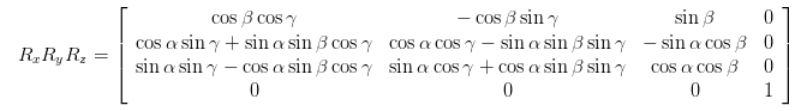
\includegraphics[width=0.9\textwidth]{rotationMatrix.jpg}
\captionof{figure}{Rotation Matrix for rotation about Z, then Y, then X axes (note: final row and column is only for translation), image from XXXX.}
\label{figure:rotationMatrix}
\end{center}

\subsubsection{Gesturing Approach for Distant Targets}
SPHERE INTERSECTION ETC.

\subsubsection{Running with a Live Target in Real Time}
RUNNING THE SET MOTOR INSTRUCTION IN A DIFFERENT THREAD IN A LOOP SO TARGET CAN BE UPDATED LIVE AND THE MOTION OF THE SERVOS IS ADJUSTED LIVE SO AS TO NOT FINISH THE PREVIOUS COMMAND AND JUST CONCENTRATE ON CURRENT TARGET.

\section{Experimental Design}
\subsection{Setup}
\subsection{Construction Environment Parallels}
\subsection{Mental Aspect}
\subsection{Physical Aspect}

\section{Results}

\section{Discussion}
\section{Conclusion}

\bibliography{mybib}
\bibliographystyle{unsrt}

\section{Appendix}
\subsection{CAD Drawings}
\end{document}